\begin{landscape}
\begin{figure}[hbt!]
\begin{center}
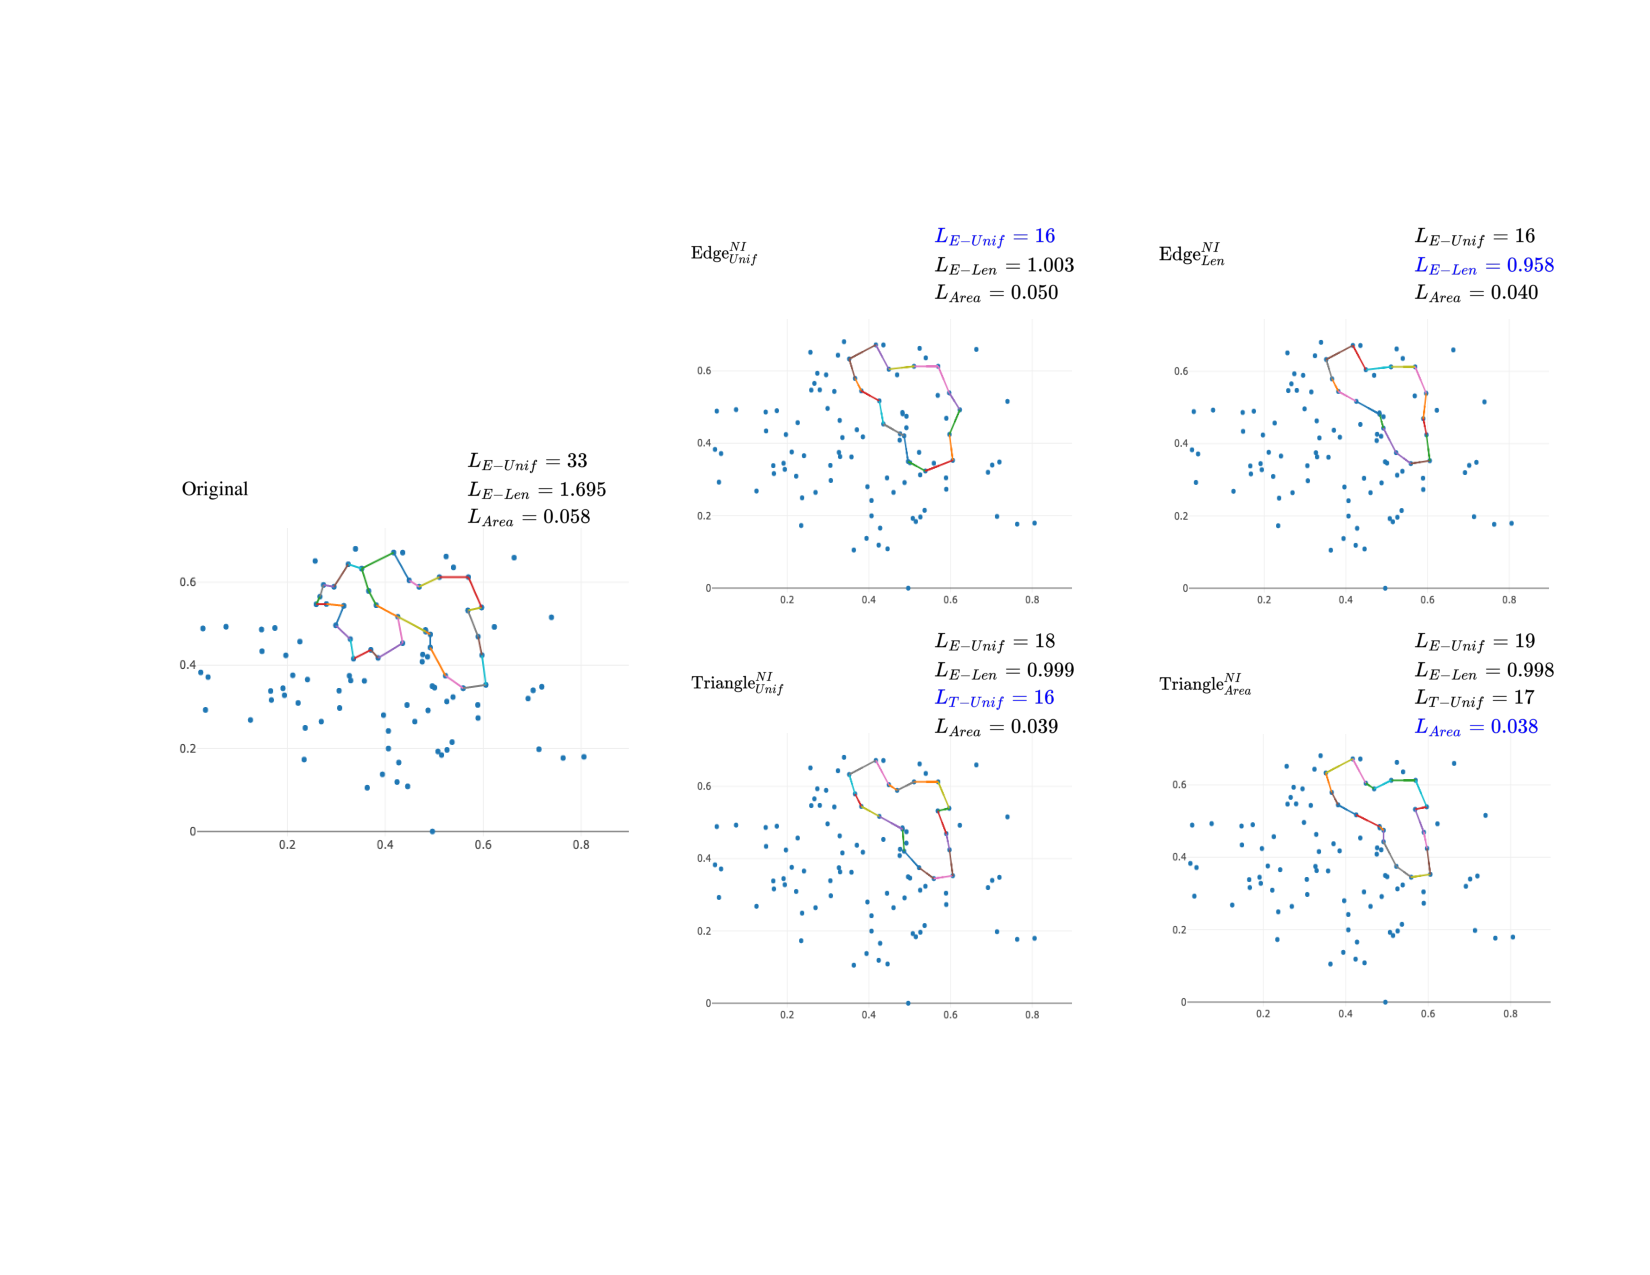
\includegraphics[width=\textwidth]{figures/examples.pdf}
\end{center}
\caption{Examples of different optimal cycles and cost against different loss functions using a point cloud of $100$ points with ambient dimension $2$ randomly drawn from a normal distribution. The upper left corner of each subfigure labels the optimization algorithm used to optimize the original cycle representative. The upper right corner of each subfigure records the different measures of the size of the optimal representative. Blue text represents the measure an algorithm sets out to optimize. 
}\label{fig:Examplesofeachoptimalcycles} 
\end{figure}
\end{landscape}
% \textbf{(A)} is the original cycle, \textbf{(B)} is the uniform-weighted minimal cycle, \textbf{(C)} is the length-weighted minimal cycle, \textbf{(D)} is the volume, \textbf{(E)} is the area optimal cycle.

% \vspace{0.1in}

% \begin{table}[hbt!]
%     \centering
%     \begin{tabular}{ |c || c |c |c |c |}
%  \hline
%  & Length & Edge  & Area & Volume  \\[0.5ex] 
%  \hline 
%  $X_{Orig}$ & 1.695 & 33  & 0.0576 &  -  \\\hline  

% $X_{Len}$ &  \textbf{0.0958} &  16  &  0.0398 &   -  \\\hline  
% $X_{Unif}$ & 1.003 & \textbf{16}   & 0.0496 &  -  \\\hline  

% $X_{Area}$ &   0.998  & 19  & \textbf{0.038 }& 17  \\  \hline
% $X_{Vol}$ &   0.999  & 18    & 0.0391 & \textbf{16} \\ \hline

% \end{tabular}
% \caption{Summary of the example in Figure \ref{fig:volumeExample}}
% \label{tab:data}
% \end{table}
